\section{Cell Nuclei Segmentation using \stardist}\label{secstardist}
As discussed in Sec.~\ref{secunsupervised}, typical instance segmentation methods suffer from the suppression of valid objects or the merging of instances given overlaps. In order to better segment the myoblasts or cell nuclei, a cell detection method called \stardist \cite{schmidt2018, weigert2020} is used. It was developed with the intent to segment microscopy data like the nuclei found in this project. A deep learning model would have the advantage of being flexible enough to not require much preprocessing and can ideally be used out-of-box if there exists a pretrained model.
\subsection{\texttt{Stardist} Background}
Cell nuclei images are characterized by their dense population, with nuclei that vary minimally in size and shape and frequently overlap. The goal of the \texttt{Stardist} developers was to define a shape that is rigid enough for consistent definition yet flexible enough to approximate cell nuclei across different contexts for prediction purposes. In brief, a convolutional neural network is trained to predict polygons imitating typical cell shapes for every pixel of the image. More concretely, it predicts a star-convex polygon for every (non-background) pixel. Intuitively speaking, a star-convex set $\mathcal{S}$ is one where there exists one point $s_{0}$ such that for every point $s \in \mathcal{S}$ the line segment connecting $s_{0}$ to $s$ is element of $\mathcal{S}$. Such a shape can be approximated by following $n$ predefined radial directions for a distance of $\{r^{k}\}^{n}_{k = 1}$ starting from a point $s_{0}$. This better approximates the shape of a cell nucleus than an ellipse does. The training data contains pairs of both raw and fully annotated images in the sense that every pixel either has a unique object identifier or is marked as background. The training of the network hinges on the estimation of two key features: object probabilities and radial distances.

Given the annotated images, for every single pixel within an object the Euclidean distance to the closest background pixel is computed. Normalizing this distance gives a value $d_{ij}$ between 0 and 1 and can be interpreted as a probability to be at the center of said object. This serves as a differentiation of background and foreground. These values will be referred to as \textbf{object probabilities}. Furthermore, it is possible to compute the \textbf{radial distances} $\{r^{k}_{ij}\}^{n}_{k = 1}$ to the boundaries of the object assigned to the pixel  starting at every single foreground pixel parametrized by $i, j$ serving as $s_{0}$. In total $n$ such radial distances radiating out with equally spaced angles are learned, where $n = 32$. The calculations are visualized in Fig.~\ref{figstardistexplained}. At the end of the day, both object probabilities and the $n$ distances are predicted for each image and denoted with $\hat{d}$ and $\hat{r}$ respectively. 

\texttt{Stardist} utilizes the \texttt{U-Net} architecture \cite{RonnebergerFB15} as its backbone, enhanced with an additional 3x3 convolutional layer featuring 128 channels and ReLU activations to increase network flexibility. This output, in turn, is then directed into two separate convolutional output layers. The first layer utilizes a single-channel convolution with sigmoid activation to learn object probabilities, which are penalized using the binary cross-entropy loss
\begin{equation}\label{eqbceloss}
	L_{\text{obj}}(d,\hat{d})=-d\log\hat{d}-(1-d)\log(1-\hat{d}).
\end{equation}
The second layer, without activation and featuring as many channels as there are radial directions, penalizes the radial distances using mean absolute error, weighted by the object probability
\begin{equation}
	L_{\text{dist}}(d,\hat{d},r_k,\hat{r}_k)=d\cdot\frac{1}{n}\sum_k|r_k-\hat{r}_k|.
\end{equation}
This weighting is pivotal, as it ensures background pixels do not contribute to the loss, and pixels closer to an object's center have a greater influence. To eliminate redundant predictions, the model employs non-maximum suppression (NMS) \cite{hosang2017learning, ren2016faster}, prioritizing polygons linked to pixels with higher probabilities.

\begin{figure}
	\centering
	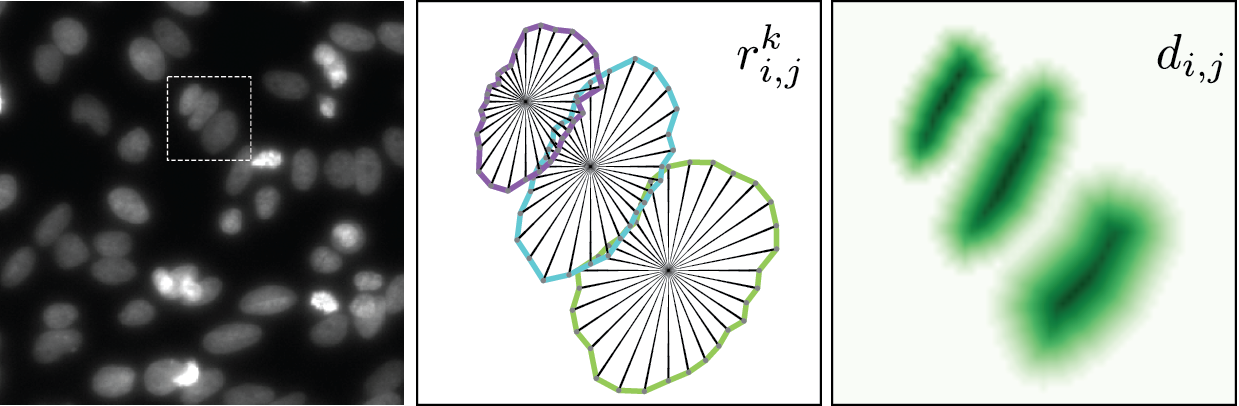
\includegraphics[width=\textwidth]{"images/star_convexity_explained.png"}
	\caption[\texttt{Stardist} summarized]{Example of an area that is complicated to segment due to overlaps. \texttt{Stardist} creates the segmentation by forming star-convex polygons and computing the probability to belong to said instance. Source: \Cite{schmidt2018}.}
	\label{figstardistexplained}
\end{figure}
